\documentclass[9pt,twocolumn,twoside]{pnas-new}
% Use the lineno option to display guide line numbers if required.
% Note that the use of elements such as single-column equations
% may affect the guide line number alignment. 

\templatetype{pnasresearcharticle} % Choose template 
% {pnasresearcharticle} = Template for a two-column research article
% {pnasmathematics} = Template for a one-column mathematics article
% {pnasinvited} = Template for a PNAS invited submission

\newcommand*{\lpath}{./}%
%\usepackage[cmex10]{amsmath, mathtools}
\usepackage{amsmath,amssymb,amsbsy,amsfonts,amsthm}
\usepackage{mathtools}
\usepackage{multirow}
\usepackage{bm}
\usepackage{enumerate}
\usepackage{url}
%\usepackage[ruled,vlined]{algorithm2e}
\usepackage{fancyvrb}
\usepackage{yfonts}
\usepackage{wrapfig}
\usepackage{tikz}
\usetikzlibrary{bayesnet}
\newcommand{\tikzmark}[1]{\tikz[overlay,remember picture] \node (#1) {};}
\usepackage{calc}%    For the \widthof macro
\usepackage{xparse}%  For \NewDocumentCommand


%% Variable de compilation
\newif\ifbeamer
\beamerfalse
\newcommand{\beamer}[2]{\ifbeamer #1 \else #2 \fi}
%%%

%\usepackage[latin1]{inputenc}
\usepackage[utf8]{inputenc} % manage utf8 encodage 
%\usepackage[english]{babel} % for french document ! dirty enumerate style,+ bad change rectangle colors for section linking.
\usepackage{fancyhdr} % for heading
\usepackage{listings}
\usepackage[colorlinks=true, urlcolor=blue]{hyperref} % url, link
\usepackage{graphicx}
\usepackage{geometry}

%\usepackage[cmex10]{amsmath, mathtools}
\usepackage{amsmath,amssymb,amsbsy,amsfonts,amsthm}
\usepackage{multirow}
\usepackage{bm}
\usepackage{enumerate}
\usepackage{url}
\usepackage[ruled,vlined]{algorithm2e}
\usepackage{fancyvrb}
\usepackage{yfonts}

\usepackage{wrapfig}
\usepackage{tikz}
    %\input{../tikz.conf}
    
\usetikzlibrary{bayesnet}
    
%%%%%%%%%%% Box 
\usepackage{calc}%    For the \widthof macro
\usepackage{xparse}%  For \NewDocumentCommand
\newcommand{\tikzmark}[1]{\tikz[overlay,remember picture] \node (#1) {};}

%%%%%%%%%% Math
\renewcommand{\text}{\textnormal}
\newcommand{\pr}{\mathbf{p}}
\newcommand{\E}{\mathbb{E}}
\newcommand{\divkk}{\mathbb{K}}
\newcommand{\entropy}{\mathbb{H}}
\newcommand{\gem}{\mathrm{GEM}}
\newcommand{\Mult}{\mathrm{Mult}}
\newcommand{\DP}{\mathrm{DP}}
\newcommand{\IBP}{\mathrm{IBP}}
\newcommand{\M}{\mathcal{M}}
\newcommand{\V}{\mathcal{V}}
\newcommand{\N}{\mathcal{N}}
    
\makeatletter
\NewDocumentCommand{\DrawBox}{s O{}}{%
    \tikz[overlay,remember picture]{
    	\IfBooleanTF{#1}{%
    		\coordinate (RightPoint) at ($(left |- right)+(\linewidth-\labelsep-\labelwidth,0.0)$);
    	}{%
    	\coordinate (RightPoint) at (right.east);
    }%
    \draw[red,#2]
    ($(left)+(-0.2em,0.9em)$) rectangle
    ($(RightPoint)+(0.2em,-0.3em)$);}
}

\NewDocumentCommand{\DrawBoxWide}{s O{}}{%
	\tikz[overlay,remember picture]{
		\IfBooleanTF{#1}{%
			\coordinate (RightPoint) at ($(left |- right)+(\linewidth-\labelsep-\labelwidth,0.0)$);
		}{%
		\coordinate (RightPoint) at (right.east);
	}%
	\draw[red,#2]
	($(left)+(-\labelwidth,0.9em)$) rectangle
	($(RightPoint)+(0.2em,-0.3em)$);}
}
\makeatother
%%%%% ! Box

\geometry{
      a4paper,
	    body={160mm,260mm},
	    left=25mm,top=20mm,
	    headheight=4mm,headsep=8mm,
        footskip=10mm,
        }
                                              

%%%%%%%%%%%%%%%%%%%%%%%%%%%%%%%%%%%%%%%%%%%%%%%%%%%%%%%%%%%%%%%%%%%%%%%%%%%%%%%%%%%%%%%%%%%%%%%%%%%%%%
%%%%% => Internal
%%%%%%%%%%%%%%%%%%%%%%%%%%%%%%%%%%%%%%%%%%%%%%%%%%%%%%%%%%%%%%%%%%%%%%%%%%%%%%%%%%%%%%%%%%%%%%%%%%%%%%

% itemize item def
%% \begin{itemize}\itemsep2pt % example space betwew item
%\renewcommand{\FrenchLabelItem}{\textbullet}
\renewcommand{\labelitemi}{$\bullet$}
\renewcommand{\labelitemii}{$\cdot$}
\renewcommand{\labelitemiii}{$\diamond$}
\renewcommand{\labelitemiv}{$\ast$}

% equation reference
\renewcommand{\theequation}{\thesection.\arabic{equation}}

%%%%%%%%%%%%%%%%%%%%%%%%%%%%%%%%%%%%%%%%%%%%%%%%%%%%%%%%%%%%%%%%%%%%%%%%%%%%%%%%%%%%%%%%%%%%%%%%%%%%%%
%%%%% => Alias
%%%%%%%%%%%%%%%%%%%%%%%%%%%%%%%%%%%%%%%%%%%%%%%%%%%%%%%%%%%%%%%%%%%%%%%%%%%%%%%%%%%%%%%%%%%%%%%%%%%%%%

% write code
\lstnewenvironment{C}[1]
{\lstset{language=C,
      frame=tBRl,
      basicstyle=\scriptsize,stringstyle=\emph,showstringspaces=false,
      numbers=left,numberstyle=\tiny,
      breaklines=true, columns=flexible, title={#1}}
}{}
      
%%%%%%%%%%%%%%%%%%%%%%%%%%%%%%%%%%%%%%%%%%%%%%%%%%%%%%%%%%%%%%%%%%%%%%%%%%%%%%%%%%%%%%%%%%%%%%%%%%%%%%
%%%%% => Preambles Pages
%%%%%%%%%%%%%%%%%%%%%%%%%%%%%%%%%%%%%%%%%%%%%%%%%%%%%%%%%%%%%%%%%%%%%%%%%%%%%%%%%%%%%%%%%%%%%%%%%%%%%%

\pagestyle{fancy}
\fancyhf{} % remove default headers
\fancyfoot[C]{\thepage}
\renewcommand{\footrulewidth}{0.3pt}
\renewcommand{\headrulewidth}{0.3pt}

%%%%%%%%%% Math
\renewcommand{\text}{\textnormal}
\newcommand{\ifm}{\texttt{ILFM}}
\newcommand{\imb}{\texttt{IMMSB}}
\newcommand{\pr}{p}
\newcommand{\p}{p}
\newcommand{\E}{\mathbb{E}}
\newcommand{\divkk}{\mathbb{K}}
\newcommand{\entropy}{\mathbb{H}}
\newcommand{\gem}{\mathrm{GEM}}
\newcommand{\Mult}{\mathrm{Mult}}
\newcommand{\DP}{\mathrm{DP}}
\newcommand{\IBP}{\mathrm{IBP}}
\newcommand{\M}{\mathcal{M}}
\newcommand{\V}{\mathcal{V}}
\newcommand{\N}{\mathcal{N}}
\newcommand{\mat}[1]{\mathbf{#1}}
\newcommand{\unit}{1\!\!1}

\newtheorem{definition}{Definition}[section]
\newtheorem{proposition}{Proposition}[section]
\newtheorem{theorem}{Theorem}[section]
\newtheorem{corollary}{Corollary}[section]


\title{Stochastic mixed membership models and link prediction: a study of homophily and preferential attachment in social networks}

% Use letters for affiliations, numbers to show equal authorship (if applicable) and to indicate the corresponding author
\author[a,b]{Adrien Dulac}
\author[a]{Eric Gaussier} 
\author[b,1]{Christine Largeron}

\affil[a]{Univ. Grenoble Alpes, CNRS, Grenoble INP, LIG - F-38000 Grenoble}
\affil[b]{Universit\'e Jean Monnet, Laboratoire Hubert Curien - F-42000 Saint-Etienne}
%\affil[c]{Affiliation Three}

% Please give the surname of the lead author for the running footer
\leadauthor{Dulac} 

% Please add here a significance statement to explain the relevance of your work
\significancestatement{We introduce formal definitions of the compliance of probabilistic link prediction models to homophily and preferential attachment in social networks, and show that standard stochastic mixed membership models comply with homophily with the similarity that underlies them. For preferential attachment, the situation is more contrasted: if these models do not comply with global preferential attachement, their compliance to local preferential attachment depends on whether the memberships to latent factors are hard or soft.}

% Please include corresponding author, author contribution and author declaration information
\authorcontributions{All authors contributed equally to the theoretical development and experimental design. A. Dulac furthermore implemented all the models and ran the experiments.}
%\authordeclaration{Please declare any conflict of interest here.}
%\equalauthors{\textsuperscript{1}A. Dulac, E. Gaussier and C. Largeron contributed equally to this work.}
\correspondingauthor{\textsuperscript{1}To whom correspondence should be addressed. E-mail: Christine.Largeron@univ-st-etienne.fr}

% Keywords are not mandatory, but authors are strongly encouraged to provide them. If provided, please include two to five keywords, separated by the pipe symbol, e.g:
\keywords{Stochastic mixed membership models $|$ Social networks $|$ Homophily $|$ Preferential attachment} 

\begin{abstract}
In this article, we assess whether standard stochastic mixed membership models are adapted to link prediction in social networks by studying how they handle homophily and preferential attachment. To do so, we introduce formal definitions of the compliance of probabilistic link prediction models to homophily and preferential attachment. Our theoretical analysis reveals that standard stochastic mixed membership models comply with homophily with the similarity that underlies them. For preferential attachment, the situation is more contrasted: if these models do not comply with global preferential attachement, their compliance to local preferential attachment depends on whether the memberships to latent factors are hard or soft. We lastly illustrate these elements on synthetic and real networks.
\end{abstract}

\dates{This manuscript was compiled on \today}
\doi{\url{www.pnas.org/cgi/doi/10.1073/pnas.XXXXXXXXXX}}

\begin{document}

% Optional adjustment to line up main text (after abstract) of first page with line numbers, when using both lineno and twocolumn options.
% You should only change this length when you've finalised the article contents.
\verticaladjustment{-2pt}

\maketitle
\thispagestyle{firststyle}
\ifthenelse{\boolean{shortarticle}}{\ifthenelse{\boolean{singlecolumn}}{\abscontentformatted}{\abscontent}}{}

\label{sec:intro}

Several powerful relational learning models have been proposed to solve the problem commonly referred to as \textit{link prediction} that consists in predicting the likelihood of a future association between two nodes in a network \cite{Liben-Nowell07, HassanZaki11}. Among such models, the class of stochastic mixed membership models has received much attention as such models can be used to discover hidden properties and infer new links in social networks. Two main models in this class have been proposed and studied in the literature: the latent feature model \cite{BMF} and its non-parametric extension \cite{ILFRM}, and the mixed-membership stochastic block model \cite{MMSB}, and its non parametric extension \cite{iMMSB,diMMSB}.

Nevertheless, although drawn from a wide range of domains, real world social networks exhibit general properties that have been put forward in different studies. In this work, we focus on two important properties, namely \textit{homophily} and \textit{preferential attachment} \cite{Newman2010, Barabasi2003}, and assess to which extent link prediction models as the ones mentioned above comply with such properties.

Stochastic mixed membership models are generative models that rely on latent factors (sometimes referred to as latent \textit{classes} or \textit{features}) that represent hidden properties of nodes, corresponding to individuals, in a graph representing the social network. They are characterized by the fact that each node can "belong" to several latent factors, which reflects the fact that each individual usually has several properties, for example can belong to several communities\footnote{As mentioned in \cite{goldenberg2010survey}, the reader should however bear in mind that the notion of latent factors is of stochastic nature and is an approximation of the notions of communities and shared properties.}. The relation between a node $i$ and the latent factors is encoded in a vector denoted $\mat{f}_{i}$, of finite dimension $K$ in standard versions of the models, and of infinite dimensions in  non-parametric versions. The collection of all vectors $\mat{f}_{i}$ ($1 \le i \le N$) constitutes the factor matrix $\mat{F}$. Furthermore, a weight matrix $\mat{\Phi}$ is used to encode correlations between the latent factors.

Stochastic mixed membership models differ on the way the vectors $\mat{f}_{i}$ ($1 \le i \le N$) and the matrix $\mat{\Phi}$ are generated. As mentioned before, and to be as general as possible, we consider here the non-parametric versions of the latent feature model \cite{ILFRM}, referred to as \ifm, and of the mixed-membership stochastic block model \cite{iMMSB,diMMSB}, referred to as \imb. In \ifm, the factor matrix $\mat{F}$ is generated by an Indian Buffet Process, and each element of the matrix $\mat{\Phi}$ is generated according to a normal distribution with 0 mean and fixed, common variance. The Indian Buffet Process yields binary vectors; the $k^{\mbox{th}}$ coordinate of the vector $\mat{f}_{i}$, denoted $f_{ik}$, is thus either $1$ or $0$, meaning that node $i$ belongs or not to the $k^{\mbox{th}}$ latent factor. In \imb, the factor matrix $\mat{F}$ is obtained with a Hierarchical  Dirichlet Process, and each element of the matrix $\mat{\Phi}$ is generated according to a Beta distribution with fixed, common parameters. The Hierarchical  Dirichlet Process yields this time membership probabilities; $f_{ik}$ directly encodes the probability that node $i$ belongs to the $k^{\mbox{th}}$ latent factor. We refer the interested reader to \cite{ILFRM} and \cite{iMMSB} for more details on these processes.

Once the factor and weight matrices have been generated, the probability to generate a link between any two nodes $i$ and $j$ for \ifm\ is given by:
%
\begin{align}
p(y_{ij}=1|\mat{F},\mat{\Phi}) = \sigma(\mat{f}_{i} \mat{\Phi} \mat{f}_{j}^\top)
\label{eq:ilfm}
\end{align}
%
where $\sigma()$ is the sigmoid function and $\top$ denotes the transpose. In \imb, one has first to select two latent factors from $\mat{f}_i$ and $\mat{f}_j$, and then generate or not a link between $i$ and $j$. This amounts to: (a) choose a class from the class membership distributions according to a categorical distribution:
%
\begin{align}
 z_{i \rightarrow j} &\sim \mbox{Cat}(\mat{f}_i) \nonumber \\
 z_{i \leftarrow j} &\sim \mbox{Cat}(\mat{f}_j) \nonumber
\end{align} 
%
and (b) generate a link with probability:
%
\begin{align}
 p(y_{ij}=1|,\mat{\Phi}) = \phi_{z_{i \rightarrow j}z_{i \leftarrow j}}
\label{eq:immsb}
\end{align}
%
where $\phi_{kk'}$ denotes the element of $\mat{\Phi}$ at row $k$, column $k'$.
%
%A graphical representation of these models is given in Figure~\ref{fig:ilfrm}.
%
%\begin{figure}[t]
%	\centering
%	\minipage{0.25\textwidth}\vspace{1cm}
%	\scalebox{0.77}{
%	\begin{tikzpicture}
  % Define nodes
  \node[obs]                      (y) {$y_{ij}$};
  \node[latent, left=1.2cm of y] (fi) {$\mat{f}_i$};
  \node[latent, right=1.2cm of y] (fj) {$\mat{f}_j$};
  \node[latent, above= of y]    (ibp) {$\mat{F}$};;
  \node[latent, below= of y, yshift=-0.3cm]   (W) {$\mat{\Phi}$};
  \node[const, left=0.7cm of ibp]   (a) {$\alpha$};
  \node[const, right=0.7cm of W]   (sw) {$\sigma_w$};

  % Connect the nodes
  \edge {fi,fj,W} {y} ;
  \edge[dashed] {ibp} {fi,fj} ;
  \edge {sw} {W} ; 
  \edge {a} {ibp} ; 

  % Plates
  \plate {yx} {(fj)(y)} {$N$} ;
  \plate[label={[label distance=-0.6cm]195:$N$}] {} {(fi)(y)(yx.north west)(yx.south west)} {} ;
  %\plate {} {(W)} {$K\times K$};
  %\plate {} {(fi)(y)(yx.north west)(yx.south west)} {$N$} ;
\end{tikzpicture}
}
%	\endminipage
%	\minipage{0.25\textwidth}
%	\scalebox{0.77}{
%    /home/dulac/Documents/workInProgress/networkofgraphs/papers/personal/figures/draw/mmsb2.tex}
%	\endminipage
%	\caption{The two graphical representations of (left) the infinite latent feature model and (right) the infinite mixed-membership stochastic block model.}
%%	The difference between the two models lies in the way representations are associated to nodes: a fixed representation is used in the case of the latent feature model, whereas the representation in the stochastic block model varies according to the link considered.}
%	\label{fig:ilfrm}
%\end{figure}

In the typical use of the above models for link prediction, some observations (\textit{i.e.} an existing network, observed till a certain time) are available and are used to estimate $\mat{F}$ and $\mat{\Phi}$, from which new links are predicted. In the remainder, we denote by $\mat{\hat{F}}$ and $\mat{\hat{\Phi}}$ the estimates of $\mat{F}$ and $\mat{\Phi}$, that are usually obtained through standard (collapsed) Gibbs sampling and Metropolis-Hastings algorithms \cite{ILFRM,IBP,HDP,diMMSB}. We furthermore denote by $\mathcal{M}_e$ the version of both \ifm\ and \imb\ in which $\mat{F}$ and $\mat{\Phi}$ are assumed known and fixed to $\mat{\hat{F}}$ and $\mat{\hat{\Phi}}$. We now investigate whether, from the learned parameters $\mat{\hat{F}}$ and $\mat{\hat{\Phi}}$, the new links generated produce a network that comply with homophily and preferential attachement.

\section{Homophily: \emph{"Birds of a feather flock together"}}
\label{sec:homophily}

Homophily refers to the tendency of individuals to connect to similar others: two individuals (and thus their corresponding nodes in a social network) are more likely to be connected if they share common characteristics~\cite{mcpherson2001birds,lazarsfeld1954friendship}. The characteristics often considered are inherent to the individuals and may represent their social status, their preferences or their interest. A related notion is the one of {\it assortativity}, that is slightly more general as it applies to any network, and not just social networks, and refers to the tendency of nodes in networks to be connected to others that are similar in some way.

A definition of homophily has been proposed in~\cite{la2010randomization}. However, this definition, which relies on a single characteristic (as age or gender), does not allow one to assess whether latent models for link prediction capture the homophily effect or not. We thus introduce a new definition of homophily below:
%
\begin{definition}[Homophily] \label{def:homophily}
	Let $\mathcal{M}_e$ be a probabilistic link prediction model and $s$ a similarity measure between nodes. We say that \emph{$\mathcal{M}_e$ is homophilic under the similarity $s$} iff, $\forall (i,j,i',j') \in V^4$:
%
\begin{equation}
s(i,j) > s(i',j')  \implies \pr(y_{ij}=1 \mid \mathcal{M}_e) > \pr(y_{i'j'}=1  \mid \mathcal{M}_e) \nonumber
\end{equation}
%
\end{definition}
%
\noindent As one can note, this definition directly captures the effect "if two nodes are more similar, then they are more likely to be connected". 

Different similarities can be considered, as long as they are based on the proximity of the properties of the nodes considered. In stochastic mixed membership models, these properties are encoded in the latent factors. Indeed, as mentioned before, the factor matrix $\mat{\hat{F}}$ aims at capturing some latent properties of the nodes, whereas the estimated matrix $\mat{\hat{\Phi}}$ captures the correlations between these latent properties. One can thus define, on their basis, a "natural" similarity between nodes as follows:
%
\begin{equation}
s_n(i,j) = \mat{\hat{f}}_{i} \mat{\hat{\Phi}} \mat{\hat{f}}_j^\top \nonumber
\end{equation}
%
It is straightforward that both \ifm\ and \imb\ in the setting $\mathcal{M}_e$ are homophilic with respect to $s_n$. Indeed, $\pr(y_{ij}=1 \mid \mathcal{M}_e)$ increases with $s_n$ for \ifm\ as the sigmoid function is strictly increasing (Eq.~\ref{eq:ilfm}). Furthermore, marginalizing over the $z$ variables in \imb\ leads to:
%
\begin{align}
\pr(y_{ij} =1 \mid \mathcal{M}_e) & = \sum_{k,k'} \hat{\phi}_{k,k'} \pr(z_{i \rightarrow j}=k | \mathcal{M}_e) \pr(z_{i \leftarrow j}=k' | \mathcal{M}_e) \nonumber \\
& = \sum_{k,k'} \hat{\phi}_{k,k'} \hat{f}_{ik} \hat{f}_{jk'} = \mat{\hat{f}}_{i} \mat{\hat{\Phi}} \mat{\hat{f}}_j^\top \nonumber
\end{align}

Dropping the correlation between latent factors in the natural similarity leads to a new similarity, solely based on the latent factors and defined by $s_l(i,j) = \mat{\hat{f}}_{i} \mat{\hat{f}}_j^\top \nonumber$ ($s_l$ stands for latent similarity). With this similarity, however, neither \ifm\  nor \imb\ are homophilic. Indeed, let us first assume that $\mat{\hat{\Phi}}$ is null on the diagonal, and strictly positive elsewhere (this can be obtained for both models). For \imb, one has:
%
\begin{align}
\pr(y_{ij}=1 \mid \M_e) & = \sum_{k' \neq k} \hat{f}_{ik} \hat{\phi}_{kk'} \hat{f}_{jk'} \nonumber 
\end{align}
%
as $\hat{\phi}_{kk} = 0$. Let us now consider $\mat{\hat{f}}_i=\mat{\hat{f}}_j=(0,1,0)$ and $\mat{\hat{f}}_{i'}=(0.5,0,0.5)$ and $\mat{\hat{f}}_{j'}=(0,1,0)$. Then, $s_l(i,j)=1$ and $s_l(i',j')=0$. However, $\pr(y_{ij}=1 \mid \M_e) = 0$ whereas $\pr(y_{i'j'}=1 \mid \M_e) > 0$. \imb\ is thus not homophilic under $s_l$. The same example, replacing $\mat{\hat{f}}_{i'}=(0.5,0,0.5)$ by $\mat{\hat{f}}_{i'}=(1,0,1)$, can be used to show that \ifm\ is neither homophilic under $s_l$.

This shows that, for a model to be homophilic, it should be designed according to the similarity at the basis of the proximity between nodes and individuals. Both \ifm\ and \imb\ have been designed on the basis the natural similarity $s_n$, and directly encode the fact that similar nodes, according to $s_n$, are more likely to connected.  It is furthermore possible to make these models homophilic under $s_l$ by imposing constraints on the weight matrix $\mat{\Phi}$ (and hence its estimate $\mat{\hat{\Phi}}$); for example, considering positive, diagonal matrices with equal values on the diagonal leads to homophilic models. In that case, the latent factors can be interpreted as community indicators, each community being of equal importance. This is in line with what is done in the study presented in \cite{AMMSB} to find overlapping communities through assortativity constraints in the mixed membership stochastic block model.

\section{Preferential attachment: \emph{"The rich get richer"}}
\label{sec:burstiness}

Preferential attachment, sometimes referred to as the \textit{rich get richer} rule, is a mechanism according to which each node is connected to an existing node with a probability that increases with the number of links of the chosen node\footnote{This property is well captured by a power law distribution, hence the claim often made that preferential attachment translates as a power law distribution for the node degrees.}. However, as noted in Leskovec \textit{et al.}, usually, in social networks, entities do not have a global knowledge of the network. The preferential attachment model is thus more likely to be local, and to be specific to communities \cite{LeskovecBKT08}.

Preferential attachment relates to a general phenomenon known as \textit{burstiness}\footnote{A.L. Barab\'asi, for example, uses the term \textit{preferential attachement} in \cite{barabasi1999emergence}, and \textit{burstiness} in \cite{barabasi_burst}.} which describes the fact that some events appear in bursts, \textit{i.e.} once they appear, they are more likely to appear again. Burstiness has been studied in different fields, in particular in computational linguistics and information retrieval to characterize word occurrences \cite{church1995poisson}. In these domains, simple definitions of burstiness, that directly capture the fact that a probability distribution is bursty if the probability of generating a new occurrence of an event increases with the number of occurrences of this event, have been proposed \cite{clinchant2008bnb,clinchant2010information}, for both discrete and continuous probability distributions. We adapt here these definitions for preferential attachment in social networks.

In the context of social networks, the notion of preferential attachement amounts to the fact that the more links a node has (\textit{i.e.} the higher its degree), the more likely it will be linked to new nodes. As mentioned before, this phenomenon however appears at different levels: globally for the whole network, and locally within classes. For global preferential attachment, the degree of a node is a known integer; for local preferential attachment, in most models, the exact degree is not known, and one has to rely on an estimate of it, as done in the following definition:
%
\begin{definition}[Preferential attachment]
Let $i$ be a node in a social network and let $d_i$ denote its degree. 
\begin{description}
 \item[(1)] \emph{Global Preferential Attachment}: we say that a probabilistic link prediction model $\mathcal{M}_e$ satisfies the global preferential attachement iff, for any node $i$, $\pr(d_i \ge n+1 \mid d_i \ge n, \mathcal{M}_e)$ increases with $n \in \mathbb{N}$;
 \item[(2)] \emph{Local Preferential Attachment}: we say that a probabilistic link prediction model $\mathcal{M}_e$ satisfies the local preferential attachement iff, for any node $i$, denoting $d_{i,k}$ the degree of node $i$ in class $k$, $\forall \epsilon \in [0,1], \, \pr(d_{i,k} \ge x+\epsilon \mid d_{i,k} \ge x, \mathcal{M}_e)$ increases with $x \in [0,N-1]$. Furthermore, $d_{i,k}$ is defined as the expectation, over all nodes in the network, of forming a link through latent factor $k$.
\end{description}
\label{def:burst-soc-net}
\end{definition}
%
As one can note, these definitions directly translate the fact that "the more connections a node has, the more likely it is to be connected to new nodes". The only difference between the local and global cases lies in the fact the degree is usually unknown in the local case, and is here estimated through its expectation.

For global preferential attachment, the degree $d_i$ directly corresponds to the number of outgoing links of node $i$. Exploiting the fact that the observations are independent given $\mat{\hat{F}}$ and $\mat{\hat{\Phi}}$, one has:
%
\begin{align}
\pr(d_{i} \ge n+1 \mid d_{i} \ge n, \mathcal{M}_e) = 1 - \prod_{j \notin \mathcal{V}(i)} P(y_{ij} = 0 \mid d_{i} \ge n, \mathcal{M}_e) \nonumber \\
= 1 - \prod_{j \notin \mathcal{V}(i)} (1 - P(y_{ij} = 1 \mid d_{i} \ge n, \mathcal{M}_e)) \nonumber
\end{align}
%
where $\mathcal{V}(i)$ denotes the set of nodes connected to node $i$. Let $c=\min_j  (1-P(y_{ij} = 1 \mid d_{i} \ge n, \mathcal{M}_e))$ (where the minimum is taken over all nodes $j$). One has:
%
\[
0 \le \pr(d_{i} \ge n+1 \mid d_{i} \ge n, \mathcal{M}_e) \le (1 - c^{N-n}) \xrightarrow[n \rightarrow N]{} 0
\]
%
which shows that $\pr(d_{i} \ge n+1 \mid d_{i} \ge n, \mathcal{M}_e)$ does not increase with $n$. We thus have the following property:
%
\begin{proposition}[]
\label{pref-attch-glob}
Both \ifm\ and \imb\ do not satisfy global preferential attachment.
\end{proposition}

For local preferential attachment, the situation is slightly more complex:
%
\begin{proposition}[]
\label{pref-attch-loc}
\imb\ satisfies local preferential attachment whereas \ifm\ does not.
\end{proposition}
%
\noindent \textbf{Proof} Let $y_{ij,k}$ be the binary random variable that is $1$ if nodes $i$ and $j$ are linked through the latent factor $k$ and $0$ otherwise. Then, $d_{i,k} = \sum_{j} \pr(y_{ij,k} =1 | \mathcal{M}_e)$. For \imb, this leads to $d_{i,k} = \sum_{j} \hat{f}_{ik} \hat{\Phi}_{kk} \hat{f}_{jk} = \hat{f}_{ik} \sum_{j \in \mathcal{V}(i)} \hat{\Phi}_{kk} \hat{f}_{jk}$. The positive reinforcement effect of the Dirichlet Process \cite{teh2006hierarchical} at the basis of \imb\ corresponds to a burstiness phenomenon and directly translates, for any $i$ and any $k$, as: $\pr(\hat{f}_{ik} \ge x'+\epsilon' \mid \hat{f}_{ik} \ge x',\mathcal{M}_e)$ increases with $x'$ (for all $\epsilon'$ and $x'$ chosen according to the domain of definition of $\hat{f}_{ik}$). Setting $x=x'(\sum_{j} \hat{\Phi}_{kk} \hat{f}_{jk})$ and $\epsilon = \epsilon'(\sum_{j} \hat{\Phi}_{kk} \hat{f}_{jk})$ and exploiting the fact that $\sum_{j} \hat{\Phi}_{kk} \hat{f}_{jk}$ is positive and independent of $i$ leads to: $\pr(d_{i,k} \ge x+\epsilon \mid d_{i,k} \ge x, \mathcal{M}_e)$ increases with $x$, which proves that \imb\ satisfies the local preferential attachment effect. For \ifm, as $\hat{f}_{ik}$ is binary, there is no positive reinforcement effect and the above reasoning does not hold. Let $C_{i,j} = |\{j, \hat{f}_{jk} = \hat{f}_{ik} = 1\}|$, where $|.|$ denotes the cardinal of a set ($C_{i,j} = 0$ if $\hat{f}_{ik} =0$). As the factor matrix is binary, one has:
%
\[ 
d_{i,k} = \sum_{j} \sigma(\hat{f}_{ik} \hat{\Phi}_{kk} \hat{f}_{jk}) =  C_{i,j} (\sigma(\hat{\Phi}_{kk}-0.5) + \frac{N}{2}
\]
%
which equals $\frac{N}{2}$ when $\hat{\Phi}_{kk} = 0$. The local degree is thus constant is this case, which shows that \ifm\ does not satisfy local preferential attachment. \hspace{4.7cm} $\Box$

The above propositions show that both models are deficient in the sense that they do not guarantee that the networks they generate will comply to the global (and local in case of \ifm) preferential attachment phenomena, which are inherent properties of the probability distributions underlying the models. This does not mean however that \ifm\ and \imb\ are not able to model well social networks during the learning phase, even according to the underlying degree distribution. Indeed, the Gibbs updates for both models will assign higher weight to nodes and factors that have been used during the learning phase. Provided there is enough training data, both models will likely reproduce the degree distributions observed in the training data. We will observe that in the following section, devoted to the illustration of the properties we have established.

\section{Illustration}
%\section{Experimentations}

To illustrate our theoretical results, we evaluate the predictive performance and the ability of the models to capture homophily and preferential attachment on artificial and real networks. In the sequel, we first describe the measures used to evaluate the properties of interest and the predictive performance, then the datasets used in our experiments. Afterwards, we detail the evaluation protocol and we present the experimental results.


\subsection{Preferential attachment Measures}
\label{sec:experiments-burst}

The measures considered to evaluate the preferential attachment rely on a goodness of fit. Indeed, it has been reported that preferential attachment leads to networks characterized by a degree distribution with heavy tail drawn from a power law \textbf{ref?}. A graphical method, most often used to verify that the observations are consistent with this law  consists in constructing the histogram representing the degree distribution and if the plot on doubly logarithmic axes approximately falls on a straight line, then one can assume that the distribution follows a power law. Thus, the comparison of the degree distribution in the log-log scale with a linear function gives us a qualitative measure for the preferential attachment. To obtain a second evaluation of the power law hypothesis for the degree distribution, we follow the statistical framework, introduced by \cite{clauset2009power}, for discerning and quantifying power-law behavior in empirical data. This framework combines maximum-likelihood fitting methods with goodness-of-fit tests based on the Kolmogorov-Smirnov statistic. It includes the following steps:


\begin{itemize}
	\item Estimate the parameters $\alpha$ and $x_\text{min}$ of the power law model. $\alpha$ is the scaling parameter of the law and $x_\text{min}$, the lower bound for the tail. This last one has been fixed to the smallest value observed in the distributions evaluated, in our experiments to allow their comparisons.
	\item  Using the Kolmogorov-Smirnov (KS) statistic, compute the distance $KS_{obs}$  between the degree distribution obtained on the network with the theoretical distribution corresponding to the power law with the estimated parameters.
	\item Sample $S$ synthetic datasets from the power law with the estimated parameters. For each sample, we are using the Kolmogorov-Smirnov statistic to compute the distance $KS_{s}$ between the distribution obtained on this synthetic dataset drawn from the power law with the corresponding theoretical distribution. The precision of the $p$-value is based on the number of samples $S$ that we fix to 275. 
    \item  The p-value is defined as the fraction of  the resulting statistics $KS_s, s \in \{1,...,S\}$  larger than the value $KS_{obs}$.  
\end{itemize}

 If  p-value is large (close to 1), then the difference between the data and the model can be attributed to statistical fluctuations alone; if it is small, the model is not a plausible fit for the data and we can not conclude that there is an evidence for the preferential attachment in the network. 
\textbf{arevoir}However, as mentioned in \cite{clauset2009power} high value of the $p$-value should be considered with caution for at least two reasons. First, there may be other distribution that match the data equally or better. Second, a small number of samples of the data may lead to high p-value and reflect the fact that is hard to rule out a hypothesis in such a case.


\paragraph{Local burstiness : }
%In the context of latent models, while there is no ambiguity in computing the overall degree distribution, it is less obvious for the local case. We explain here the computation of the local degree distribution for each models according to section \ref{sec:burstiness} :
The computation of the local degree distribution for each model defined according to section \ref{sec:burstiness} is detailed below: 
\begin{itemize}
        \item For each network learned with IMMSB, the tensor $Z$ indicates the membership of the nodes for each  interaction. In order to draw the local degree distribution for a factor $k$, we reduce the adjacency matrix in order to retain only the links that occur for the factor $k$. The local degree distribution is thus computed on the reduced adjacency matrix  $Y^k =\{ y_{ij}^k=1 \ \textrm{if}\ y_{ij}=1 , z_{i\rightarrow j}=k, z_{i\leftarrow j}=k\}$. \textbf{termes a 0}
       \item for ILFM, each node $i$ is associated with a fix feature vector $\mat{f}_{i}$ ; the local degree distribution for the factor $k$ is obtained by taking into account only the contribution of this feature $k$ on the adjacency matrix. Thus, the local degree degree distribution is computed on the reduced adjacency matrix defined by $Y^c =\{ y_{ij}^c=1 \ \textrm{if}\ y_{ij}=1 , f_{ic}=1, f_{jc}=1\}$. \textbf{termes a 0}
\end{itemize}

\subsection{Homophily Measures}


For the homophily property, defined in section \ref{sec:homophily}, we represent using a box plot, for each model and each data set, the distributions of the similarity natural $s_n(i,j)$ and latent $s_l(i,j)$ computed respectively on linked and non-linked pairs of nodes for 10 networks generated with the model learned on the dataset.
% The links or non-links are obtained by running the models in a generative mode. For each models we aggregated  the similarity of each couple of nodes as well as link prediction (links or non-links). The distributions of similarities are then represented on a boxplot that shows how the they are spread according to links and non-links.


\subsection{Prediction performance evaluation}
The prediction problem is equivalent to a binary prediction problem within two classes since it consists to decide for each pair of nodes if there is an edge or not between them. 
Thus, the performance of the models can be evaluated with usual AUC-ROC measures: Receiver operating characteristic curves allow to graphically compare the predictive performance of the models on each datasets.

\subsection{Training Datasets}

In our experiments, we consider two artificial networks and two real networks.  Main topological characteristics of these networks are summarized in Table \ref{table:networks_measures} and we describe those networks in the sequel.

\begin{table}[h] 
	\centering
	\caption{Characteristics of artificial and real networks.}
	%\resizebox{\textwidth}{!}{  
    \begin{tabular}{lrrr}
        \hline
        \textbf{Networks} &   nodes &   edges &   density \\
        \hline
        Network 1 &    1000 &    3507 &     0.007 \\
        Network 4 &    1000 &   31000 &     0.062 \\
        Blogs         &    1490 &   20512 &     0.009 \\
        Manufacturing &     167 &    5950 &     0.215 \\
    \hline
    \end{tabular}
	\label{table:networks_measures}
\end{table}

The artificial networks (Network1 and Network4) \textbf{Revoir Network 4 en Network 2} have been generated with DANCer-Generator \cite{largeron2015}. This generator has been chosen because it allows to build an attributed graph having a community structure  and  the known properties of real-world networks such as preferential attachment and homophily.
Moreover, by modifying the parameters, these properties can be weakened. Finally, DANC-Generator is available under the terms of the GNU Public License and the parameters can be shared for experiments reproducibility. \textcolor{red}{Heeere, words about my platform (pymake) to share and reproduce and create new experiments}.

We evaluated also the models on two real world networks.
The first one, denoted Blogs \footnote{available at: http://moreno.ss.uci.edu/data.html\#blogs}, contains front-page hyperlinks between blogs in the context of the 2004 US election. A node represents a blog and an edge represents a hyperlink between two blogs.
The second one, denoted Manufacturing \footnote{available at: https://www.ii.pwr.edu.pl/~michalski/index.php?content=datasets\#manufacturing}, is an internal email communication network between employees of a mid-sized manufacturing company. Each vertex is associated  to an employee and an oriented link represents like previously a sent email. We can noticed that Manufacturing is specific since it is a firm's network where the relationships between the employees are constrained. 


The adjacency matrices and global degree distributions of these networks are presented in Figure \ref{fig:corpuses} whereas Figure \ref{fig:synt_graph_local} represents the local degree distribution. In this last figure, the inner degree distribution (edges inside a community) and outer degree distribution (edges between community) are plotted separately for each network. The first section of Table \ref{table:me_gofit} (Empirical) reports the resulting $p$-value of the KS test as well as the value estimated for the parameter  $\alpha$ in the global case (right) and in the local case (left). As the ground truth is not available for the real networks (Blogs and Manufacturing), communities have been determined with Louvain algorithm ( \textbf{ref}) and, the local distribution defined according to the obtained communities. 

These networks present  different affinity with the preferential attachment effect.
Indeed, As shown Figure \ref{fig:corpuses}, Network1 and Blogs verify the  global preferential attachment whereas it is not the case for Network4 and Manufacturing. The results of the KS test given in Table \ref{table:me_gofit} confirm this analysis since the $p$-value equals 1 for Network1 and Manufacturing whereas it is null for Network4, and Manufacturing.

The local degree distributions per classes, presented in Figure \ref{fig:synt_graph_local}, and the average results (and standard deviation) for the p-value computed over the communities reported, in Table \ref{table:me_gofit}, lead to the same conclusion concerning the local preferential attachment which is well verified for Network 1 and Blogs with a p-value equals to 1 but in a lesser extend for Network 4 and Manufacturing with respectively a p-value equals to 0.6 and 0.5. \textbf{pas d'acc avec la suite de ton commentaire} \textcolor{red}{j'ai modifié, c'est mieux?} We notably observe that there is a high variance of the $p$-value for Network4 and Manufacturing, which indicates that the property varies among the classes for those networks. Thus, for the preferential attachment property, global and local, we can distinguished both Network 1 and Blogs to satisfy the preferential attachment from Network4 and Manufacturing who are not. 

\textbf{quid homophily?}


\begin{figure}[h]
        \begin{minipage}{0.24\textwidth}
            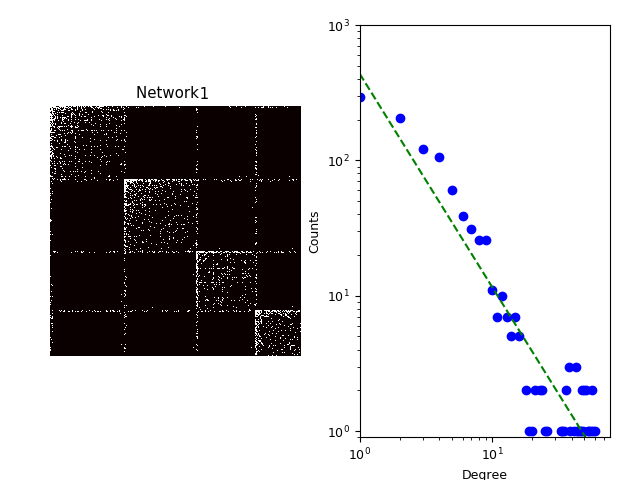
\includegraphics[width=\textwidth]{img/corpus/network1_dd}
        \end{minipage}
        \begin{minipage}{0.24\textwidth}
            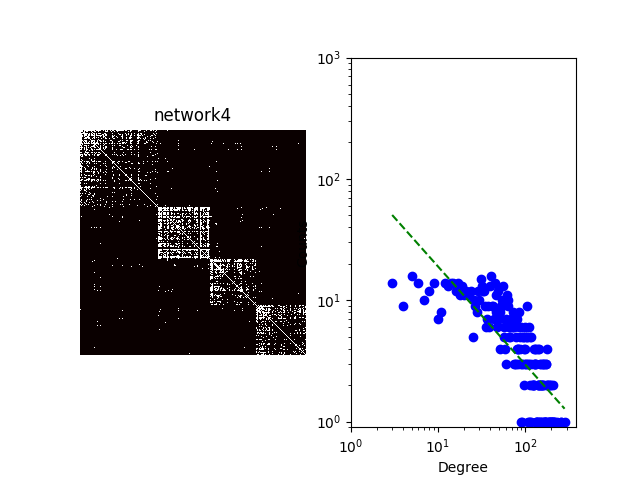
\includegraphics[width=\textwidth]{img/corpus/network4_dd}
        \end{minipage}
        \vskip\baselineskip
        \begin{minipage}{0.24\textwidth}
            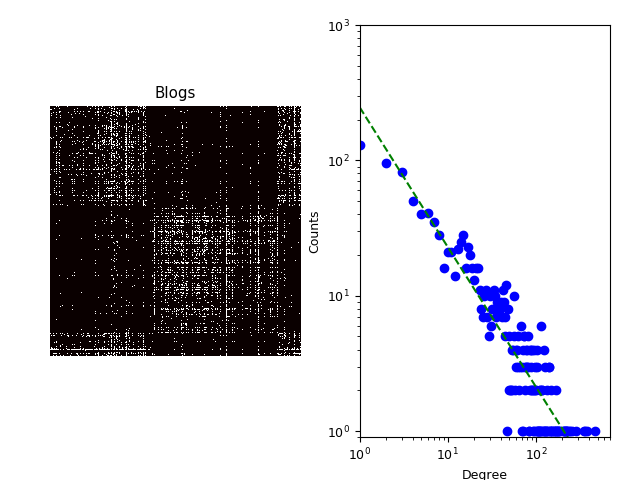
\includegraphics[width=\textwidth]{img/corpus/blogs_dd}
        \end{minipage}
        \begin{minipage}{0.24\textwidth}
            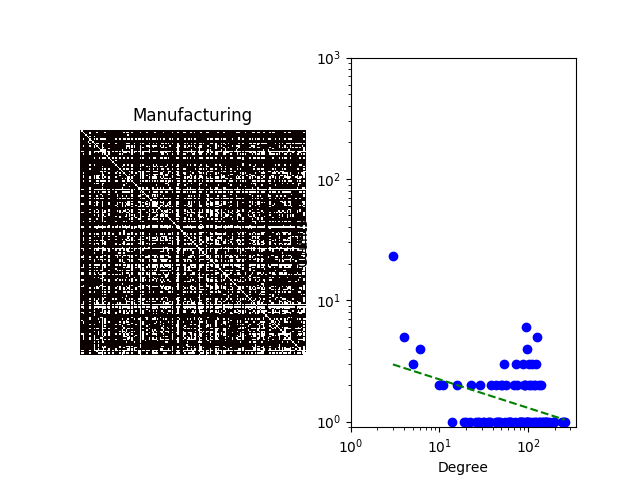
\includegraphics[width=\textwidth]{img/corpus/manufacturing_dd}
        \end{minipage}
	\caption{Adjacency matrices (left) and global degree distributions (right) for the networks datasets.}
	\label{fig:corpuses}
\end{figure}


\begin{figure}[h]
        \begin{minipage}{0.24\textwidth}
            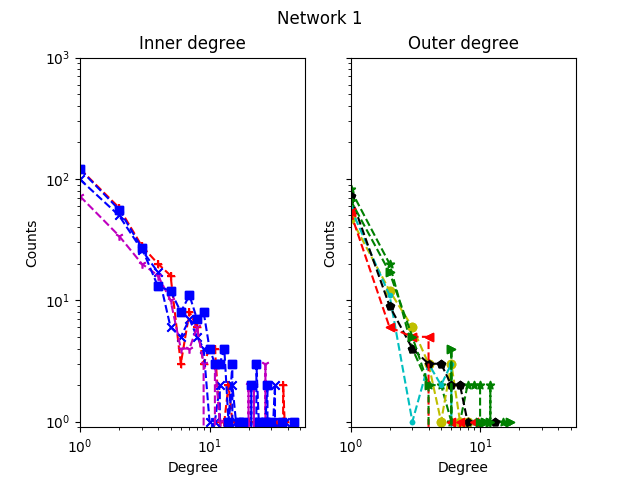
\includegraphics[width=\textwidth]{img/corpus/network1_1}
        \end{minipage}
        \begin{minipage}{0.24\textwidth}
            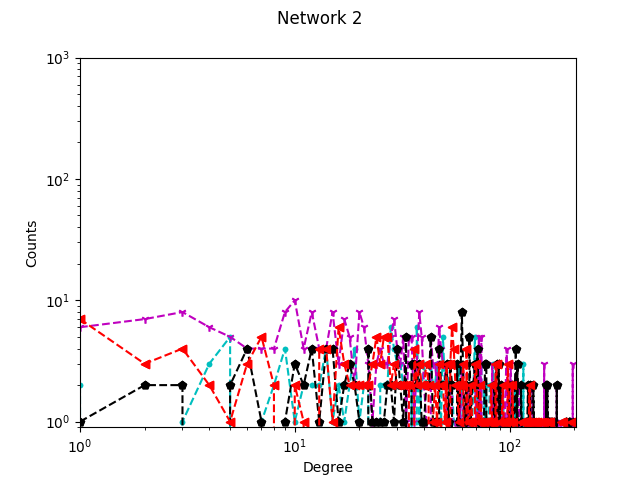
\includegraphics[width=\textwidth]{img/corpus/network2_1}
        \end{minipage}
        \vskip\baselineskip
        \begin{minipage}{0.24\textwidth}
            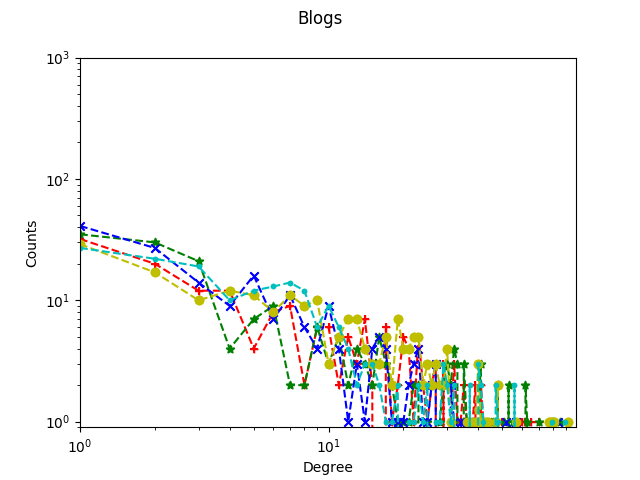
\includegraphics[width=\textwidth]{img/corpus/blogs_1}
        \end{minipage}
        \begin{minipage}{0.24\textwidth}
            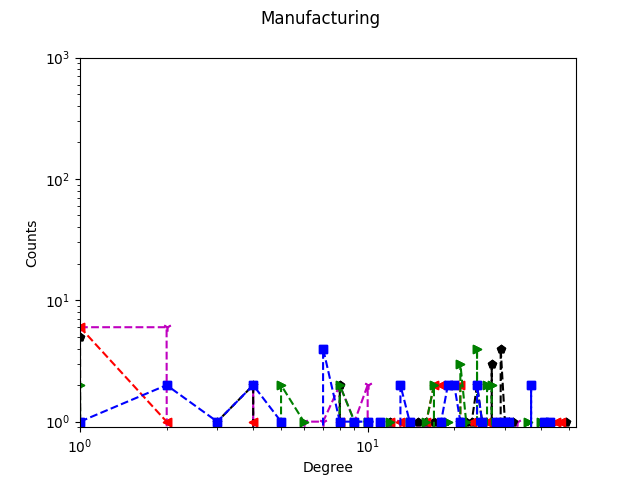
\includegraphics[width=\textwidth]{img/corpus/manufacturing_1}
        \end{minipage}
        \caption {Local degree distributions for the four networks datasets. Inner(left) and outer(right) degree are separated. For Network1 and Network2 the classes come from ground-truth. For Blogs and Manufacturing we use classes find by a Louvain algorithms.} 
	\label{fig:synt_graph_local}
\end{figure}




\subsection{Model Evaluation}
For each dataset described earlier, we run a MCMC inference consisting of 200 iterations to learn the posterior distribution for the IMMSB and ILFM  models described in section \ref{sec:models}. For IMMSB, the concentration parameters of HDP were optimized according to \cite{HDP} using vague gamma priors $\alpha_0 \sim \text{Gamma}(1,1)$ and $\gamma \sim \text{Gamma}(1,1)$. The parameters for the matrix weights were fixed to $\lambda_0=\lambda_1=0.1$. For ILFM, the IBP hyper-parameter was fixed to $\alpha=0.5$ and the weights hyper-parameter to $\sigma_w = 1$. 

The inference procedure was run with these settings for the four datasets previously described and we present hereafter the averaged results (and standard deviations) computed on ten networks generated with the model fitted for each dataset.

\textbf{mettre ailleurs}All our experimental platform is available online \footnote{https://github.com/dtrckd/pymake}. It is an ongoing development in order to provide a flexible way to design, make and share and experiments for data analysis in order to improve the ability of the community to do reproducible research.

Table \ref{table:me_gofit} reports the value of the power-law goodness of fit for IMMSB and ILFM in the global case (right) and in the local case (left). It appears that for the both models, the global preferential attachment is only verified in the generated networks learned from datasets where the property was verified, namely in Network 1 with p-value equals to 0.9 for IMMSB and 1 for ILFM, and in Blogs with a p-value equals to 1 for the both models whereas the property is not verified in Network 4 and in Manufacturing (p-value = 0). This is in accordance with Proposition 2.1 \textbf{mettre ref} according which both ILFM and IMMSB do not satisfy global preferential attachment. However these models are able to capture this property if it exists in the learning dataset.  Moreover we can observed that, in the local case, IMMSB complies with the preferential attachment with a maximal p-value for the four networks while ILFM obtained low p-values for the networks that were less locally bursty with a value of 0.5 and 0.3 respectively for Network4 and Manufacturing. \textbf{que conclue tu de la phrase suivante} \textcolor{red}{Donc que plus alpha est proche de (loi constante) moins le burstiness est significatif...} Also, the mean value of the power-law coefficient $\alpha$ is significantly greater for IMMSB than for ILFM for the different datasets with stronger values for the strongest locally bursty networks Network1 and Blogs.

The figure \ref{fig:me_local} illustrates the local preferential attachments by plotting the average local degree distribution for the artificial networks \textbf{average pas trrivial ?}  Network1 (left) and Network4 (right) learned with IMMSB (top) and ILFM (bottom). The shape of local degree distribution appears more bursty for IMMSB and with more fluctuations for ILFM which can be explained by the deficiency of ILFM to comply with local preferential attachment property as demonstrated in Proposition 2.2 \textbf{ref}.
 
 

\begin{table}[t]
    \caption{Power law goodness of fit results for the preferential attachment for empirical data and fitted models.}
\centering
  \begin{tabular}{lrrrr}
      \multirow{2}{*}{\textbf{Empirical}}  &
      \multicolumn{2}{c}{Global} & \multicolumn{2}{c}{Local}\\
      \cmidrule(r){2-3} \cmidrule(l){4-5}
      &   $p$-value &   $\alpha$   & $p$-value & $\alpha$   \\
  	\hline
    Network 1     &    1.0 &   2.4 & 1.0 $\pm$ 0.0  &  2.4 $\pm$ 0.5  \\
    Network 4     &    0.0 &   1.3 & 0.6 $\pm$ 0.5  &  1.5 $\pm$ 0.2 \\
    Blogs         &    1.0 &   1.5 & 1.0 $\pm$ 0.   &  1.7 $\pm$ 0.3 \\
    Manufacturing &    0.0 &   1.4 & 0.5 $\pm$ 0.2  &  1.4 $\pm$ 0.1 \\
  	\hline

      \ \textbf{IMMSB} &&&& \\
  	\hline
    Network 1     & 0.9 \(\pm\) 0.1   & 1.4 \(\pm\) 0.0 & 1.0 \(\pm\) 0.0   & 2.9 \(\pm\) 1.4 \\
    Network 4     & 0.0 \(\pm\) 0.0   & 1.3 \(\pm\) 0.1 & 1.0 \(\pm\) 0.0   & 1.8 \(\pm\) 0.2 \\
    Blogs         & 1.0 \(\pm\) 0.0   & 1.3 \(\pm\) 0.0 & 1.0 \(\pm\) 0.0   & 4.5 \(\pm\) 0.9 \\
    Manufacturing & 0.0 \(\pm\) 0.1   & 1.2 \(\pm\) 0.0 & 1.0 \(\pm\) 0.1   & 1.8 \(\pm\) 0.2 \\
  	\hline

      \ \textbf{ILFM} &&&& \\
  	\hline
    Network 1     & 1.0 \(\pm\) 0.0 & 1.4 \(\pm\) 0.0 & 1.0 \(\pm\) 0.0 & 1.8 \(\pm\) 0.3 \\
    Network 4     & 0.0 \(\pm\) 0.0 & 1.2 \(\pm\) 0.0 & 0.5 \(\pm\) 0.5 & 1.3 \(\pm\) 0.1 \\
    Blogs         & 1.0 \(\pm\) 0.0 & 1.3 \(\pm\) 0.0 & 1.0 \(\pm\) 0.0 & 1.5 \(\pm\) 0.1 \\
    Manufacturing & 0.0 \(\pm\) 0.0 & 1.2 \(\pm\) 0.0 & 0.3 \(\pm\) 0.3 & 1.3 \(\pm\) 0.0 \\
  	\hline
  \end{tabular}
\label{table:me_gofit}
\end{table}

\begin{figure}[h]
        \begin{minipage}{0.24\textwidth}
            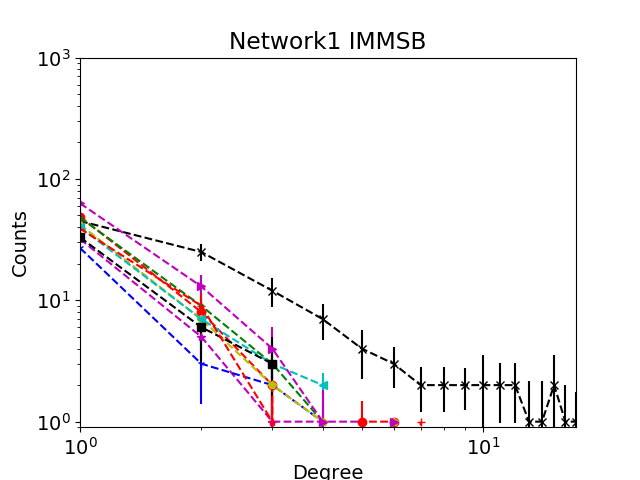
\includegraphics[width=\textwidth]{img/corpus/immsb_network1_1}
        \end{minipage}
        \begin{minipage}{0.24\textwidth}
            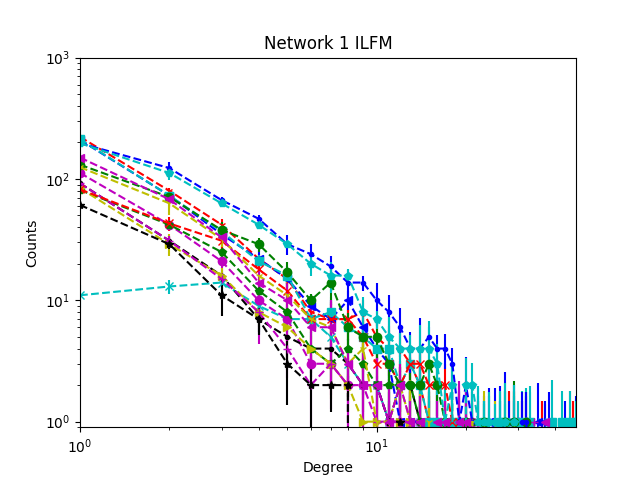
\includegraphics[width=\textwidth]{img/corpus/ilfm_network1_1}
        \end{minipage}
        \vskip\baselineskip
        \begin{minipage}{0.24\textwidth}
            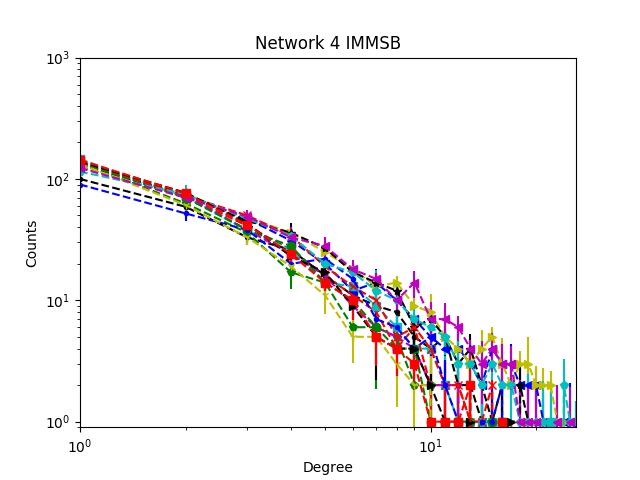
\includegraphics[width=\textwidth]{img/corpus/immsb_network4_1}
        \end{minipage}
        \begin{minipage}{0.24\textwidth}
            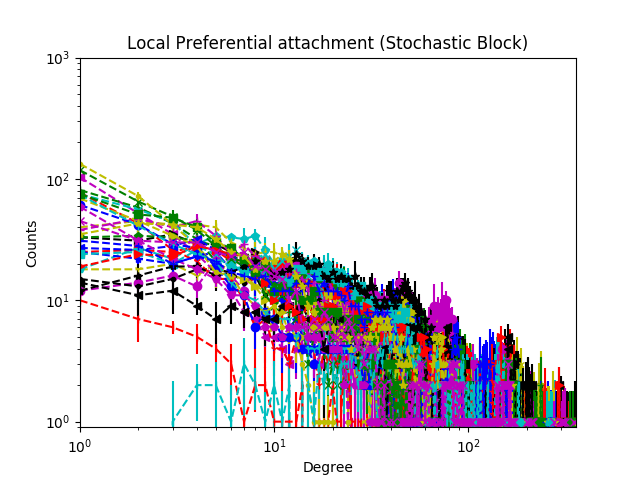
\includegraphics[width=\textwidth]{img/corpus/ilfm_network4_1}
        \end{minipage}
        \caption {Local degree distribution for of fitted models for Network 1 (first column) and Network 4 (second column) learned by IMMSB (row 1) and ILFM (row 2).} 
	\label{fig:me_local}
\end{figure}

Figure \ref{fig:homo_mustach} presents box plots describing  the distributions of the similarity natural $s_n(i,j)$ and latent $s_l(i,j)$ computed respectively on linked and non-linked pairs of nodes for 10 networks generated with IMMSB (left) and ILFM (right). We aggretated the results for all four datasets.  It confirms that the natural similarity is  higher for  pairs of nodes which are connected than between nodes which are not linked for both models. However, we can noticed that for IMMSB, the similarities computed on the non linked pairs are more concentrated around zero which is an interesting insight of the bursty behavior of this model. For the latent similarity,  there is no difference between the linked and not linked pairs, and consequently, we can not say that similar nodes are more likely to be connected. These experimental results are in accordance with our theoretical results presented in Section \textbf{ref} which states that both ILFM and IMMSB are homophilic with respect to the natural similarity $s_n(i,j)$ and are not homophilic for the latent similarity $s_l(i,j)$ .

\begin{figure}[h]
    \centering
        \begin{minipage}{0.24\textwidth}
            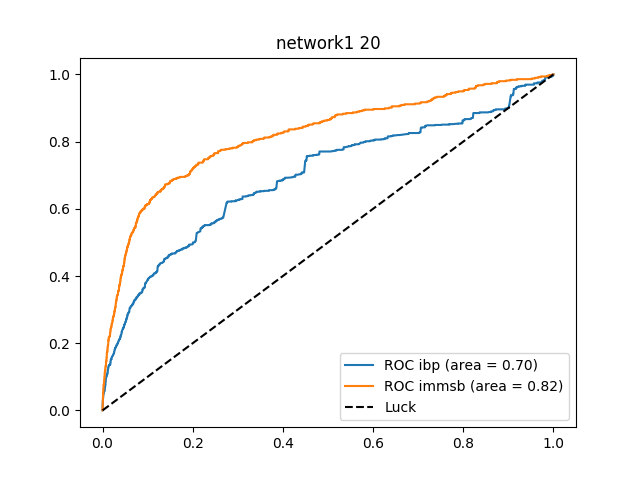
\includegraphics[width=\textwidth]{img/corpus/roc_network1_20}
        \end{minipage}
        \begin{minipage}{0.24\textwidth}
            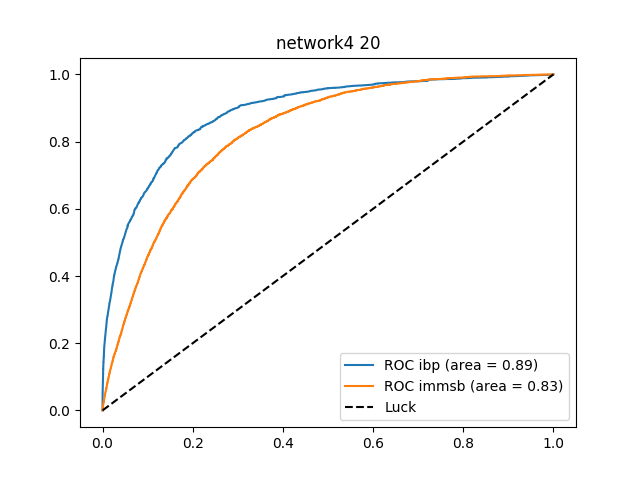
\includegraphics[width=\textwidth]{img/corpus/roc_network4_20}
        \end{minipage}
        \begin{minipage}{0.4\textwidth}
            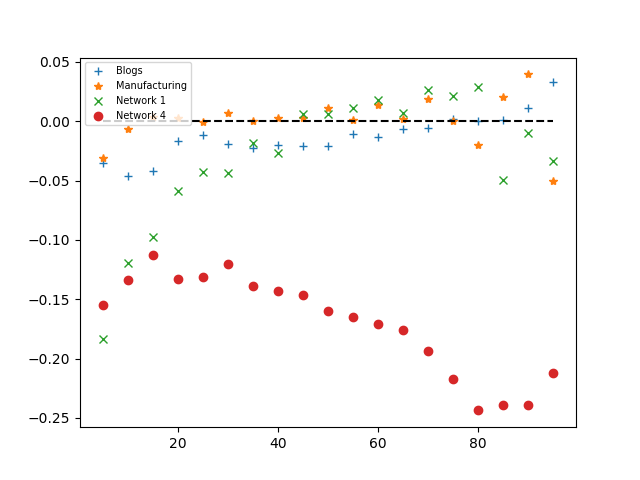
\includegraphics[width=\textwidth]{img/corpus/testset_max_20_roc_evolution.png}
        \end{minipage}
        \caption{The two upper top figures represent AUC-ROC curves that compares ILFM and IMMSB on network 1 and network4. The bottom figure is the relative AUC values when the size of the traning set vary from 10 to 95 percent. } 
	\label{fig:auc}
\end{figure}


Figure \ref{fig:auc}, compares the performances of the models on the different datasets in function of  the training set size. Indeed, in this Figure, the y-axis gives the relative performance defined as the difference of the AUC values obtained for IMMSB and ILFM: $AUC_{IMMSB} - AUC_{ILFM}$ and the x-axis represents the following ratio $\frac{testset\ size}{training\ size}$. Hence the number of training data decreases with the x-axis and a positive value on the y-axis indicates that IMMSB outperforms ILFM. 

For the artificial networks Network1 and Network 4, it is clear that IMMSB dominates ILFM on the first one, which is bursty, and is being dominated on the second one, which is not bursty.

More generally, it seems that for bursty networks, the predictive performance of IMMSB increases when the quantity of training data decreases whereas for non-bursty networks, the results are the opposite: the performance of ILFM increases when the size of the learning data decreases. This is particularly visible for Network4. For manufacturing, it is more contrasted, probably due to the fact that the size of this network is quite small which makes the comparison more difficult.


\begin{figure}[h]
    \centering
        \begin{minipage}{0.24\textwidth}
            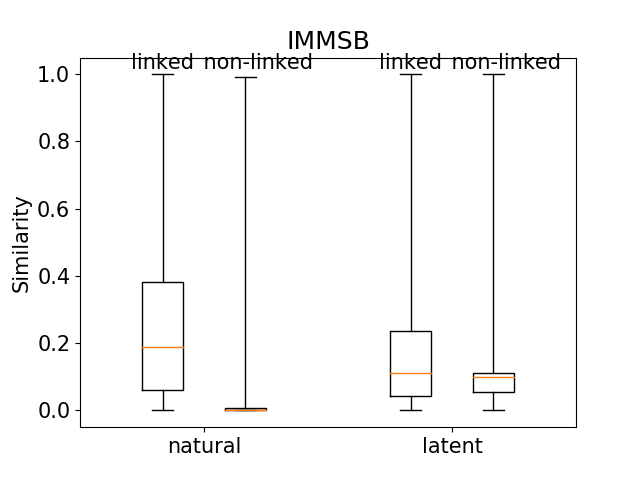
\includegraphics[width=\textwidth]{img/corpus/homo_mustach_immsb}
        \end{minipage}
        \begin{minipage}{0.24\textwidth}
            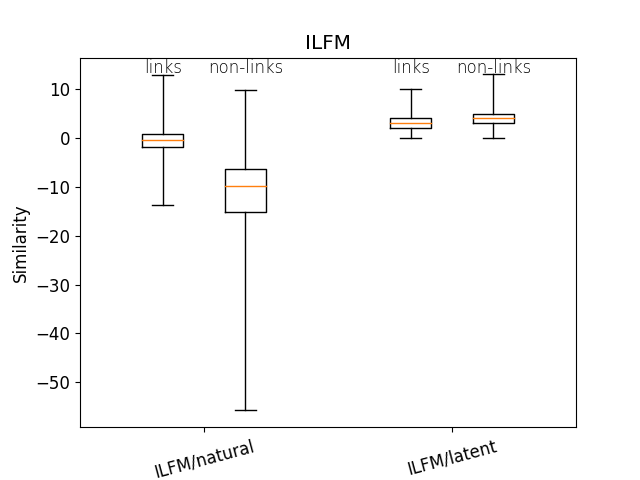
\includegraphics[width=\textwidth]{img/corpus/homo_mustach_ilfm}
        \end{minipage}
        \caption{Box plot for IMMSB (left) and ILFM (left) of the distributions for natural and latent similarities on the overall datasets. }
        \label{fig:homo_mustach}
\end{figure}




\section{Conclusion}
In this article, our aim was to study whether stochastic mixed membership models such as ILFM and IMMSB can generate networks having  properties frequently verified in real  social networks, namely  homophily and preferential attachment. 
In this aim, we have introduced formal definitions of  these properties and  analysis the behavior of these models in this theoretical  framework. We have shown that the models satisfy the homophily with the similarity that underlies them but, that it is not the case for the natural similarity. 

Concerning the preferential attachment, the models do not comply with the preferential attachment, defined on the whole network. However, the situation is more contrasted when the property is considered at the local level. In that case, we shown that IMMSB complies the property whereas ILFM does not.

Finally, experiments done on real and artificial networks have been presented to illustrate our theoretical results. They show that even if there is not a theoretical guarantee that the networks generated  have the  properties, these models are able to generate networks verifying these both properties if they are  strongly present in the dataset used to learn the model.

% In this paper we study two fundamentals properties that arise in social networks in the spectrum of Bayesian models. We proposed a probabilistic formalization of those properties and analyze how models comply with it. We showed how two families of models characterized by they prior on some latent features can conduct either to comply or not with the local preferential attachment as well as the behavior of the homophily within two appropriate similarities. This results give insight on the relation between the quality of a link prediction models and properties arising in social networks (Preferential attachment and homophily). To conclude, we think take one can take advantage of this study to better choose and design models depending on prior knwoledge on the data.

%\bibliographystyle{unsrt}
\bibliography{./pnas}

\end{document}
